% Type of the document
\documentclass[11pt]{beamer}

% elementary packages:
\usepackage{graphicx}
%\usepackage[latin1]{inputenc}
\usepackage[T1]{fontenc}
\usepackage[vietnamese]{babel}
%\usepackage[utf8]{vietnam} 
\usepackage{listings}
\usepackage{xcolor}
\usepackage{eso-pic}
\usepackage{mathrsfs}
\usepackage{url}
\usepackage{amssymb}
\usepackage{amsmath}
\usepackage{multirow}
\usepackage{hyperref}
\usepackage{booktabs}
\usepackage{tikz}
\usetikzlibrary{arrows.meta}
\usepackage{xcolor}
\usepackage{bm}
\usepackage{enumitem}

\newcommand*{\B}[1]{\ifmmode\bm{#1}\else\textbf{#1}\fi}



% additional packages
\usepackage{bbm}

% packages supplied with ise-beamer:
\usepackage{cooltooltips}
\usepackage{colordef}
\usepackage{beamerdefs}
\usepackage{lvblisting}

% Mathematics
\usepackage{amssymb}
\usepackage{amsmath}
\usepackage{mathrsfs}
\usepackage{amsthm,amsfonts}
\usepackage{mathtools}
\usepackage{algorithmic}
\usepackage[linesnumbered,ruled]{algorithm2e}
\usepackage{float}
\newcommand{\ra}{\rightarrow}
\newcommand{\Ra}{\Rightarrow}
\newcommand{\lra}{\longrightarrow}
\newcommand{\Lra}{\Longrightarrow}
\newcommand{\la}{\leftarrow}
\newcommand{\La}{\Leftarrow}
\newcommand{\lla}{\longleftarrow}
\newcommand{\Lla}{\Longleftarrow}
\newcommand{\Llra}{\Longleftrightarrow}
\newcommand{\map}{\longmapsto}
\newcommand{\al}{\alpha}
\newcommand{\bt}{\beta}
\newcommand{\dt}{\delta}
\newcommand{\De}{\Delta}
\newcommand{\tta}{\theta}
\newcommand{\e}{\varepsilon}
\newcommand{\vp}{\varphi}
\newcommand{\na}{\nabla}
\newcommand{\pa}{\partial}
\newcommand{\sm}{\sigma}
\newcommand{\Sm}{\Sigma}
\newcommand{\Gm}{\Gamma}
\newcommand{\gm}{\gamma}
\newcommand{\Om}{\Omega}
\newcommand{\R}{\mathbb R}
\newcommand{\Q}{\mathbb Q}
\newcommand{\N}{\mathbb N}
\newcommand{\Z}{\mathbb Z}
\newcommand{\Oo}{\mathcal O}
\newcommand{\K}{\mathcal K}
\newcommand{\G}{\mathcal G}
\newcommand{\D}{\mathcal D}
\newcommand{\X}{\mathcal X}
\newcommand{\M}{\mathcal M}
\newcommand{\T}{\mathcal T}
\newcommand{\V}{\mathcal V}
\newcommand{\W}{\mathcal W}
\newcommand{\PP}{\mathcal P}
\newcommand{\QQ}{\mathcal Q}
\newcommand{\UU}{\mathcal U}
\newcommand{\LL}{\mathcal L}
\newcommand{\cbe}{\scriptsize}
\newcommand{\On}{\widetilde{\mathcal{O}}}
\newcommand{\Mn}{\widetilde{M}}
\newcommand{\wt}[1]{\widetilde #1}
\newcommand{\sumh}{\overline{\sum}}
\newcommand{\cho}[2]{\ensuremath{#1\choose#2}}
\newcommand{\ve}[1]{{\bf #1}}

\DeclareMathOperator{\Div}{div}
\DeclareMathOperator{\Vol}{Vol}
\DeclareMathOperator*{\argmin}{argmin}
\DeclarePairedDelimiter{\norm}{\lVert}{\rVert}
\DeclarePairedDelimiter{\abs}{\lvert}{\rvert}

\newtheorem{Not}{Notation}
\newtheorem{Hypo}{Hypothesis}
\newtheorem{Theo}{Theorem}%[section]
\newtheorem{Prop}{Proposition}%[section]
\newtheorem{Coro}{Corollary}%[section]
\newtheorem{Algo}{Algorithm}

\theoremstyle{definition}
\newtheorem{Defi}{Definition}%[section]

\theoremstyle{plain}
\newtheorem{Lem}{Lemma}%[section]
\theoremstyle{plain}
\newtheorem{Assu}{Assumption}
\usepackage[backend=biber,style=numeric, citestyle=ieee]{biblatex}
\addbibresource{sample.bib}
\theoremstyle{remark}
\newtheorem*{Rem}{Remark}
%\usepackage{caption}
\usepackage{subcaption}


% Change the pictures here:
% logobig and logosmall are the internal names for the pictures: do not modify them. 
% Pictures must be supplied as JPEG, PNG or, to be preferred, PDF
\pgfdeclareimage[height=3cm]{logobig}{Figures/logoptit}
% Supply the correct logo for your class and change the file name to "logo". The logo will appear in the lower
% right corner:
\pgfdeclareimage[height=1cm]{logosmall}{Figures/logoptit}

% Title page outline:
% use this number to modify the scaling of the headline on title page
\renewcommand{\titlescale}{1.0}
% the title page has two columns, the following two values determine the percentage each one should get
\renewcommand{\titlescale}{1.0}
\renewcommand{\leftcol}{0.6}

% smaller font for selected slides
\newcommand\Fontvi{\fontsize{10}{7.2}\selectfont}
\newcommand\Fontsm{\fontsize{8}{7.2}\selectfont}
%\usepackage{caption}

% Define the title. Don't forget to insert an abbreviation instead 
% of "title for footer". It will appear in the lower left corner:
\title[ \footnotesize  \textcolor{red}{\bf Đồ án tốt nghiệp} -- \textcolor{blue}{Trần Xuân Độ }]{\Large  \bf ĐỒ ÁN TỐT NGHIỆP ĐẠI HỌC}


% Define the authors:
\authora{\bfseries \textcolor{blue}{\Large Chủ đề: Bao lồi xấp xỉ, bao lồi trực giao và ứng dụng trong việc định hướng và phát hiện đối tượng có hướng}\vspace{20pt}} % a-c

\authorb{ Giảng viên hướng dẫn: Nguyễn Kiều Linh}
\authorc{Sinh viên thực hiện: Trần Xuân Độ - B19DCCN183 \\ 
	\hspace{3.6cm} Đặng Thị Thoa - B19DCCN676} 

% Define the institute:
\institute{\bf  Hà Nội, tháng 12 năm 2023}

% Comment the following command, if you don't want, that the pdf file starts in full screen mode:
\hypersetup{pdfpagemode=FullScreen}

%%%%
% Main document
%%%%
\setbeamertemplate{section in toc}[square]
\setbeamertemplate{subsection in toc}[ball unnumbered]
\AtBeginSection[]
{
	\begin{frame}
		\frametitle{Nội dung chính}
		\tableofcontents[currentsection]
	\end{frame}
}% mỗi đầu section thì thêm 1 frame mục lục làm nổi bật section đó%
\AtBeginSubsection[]
{
	\begin{frame} 
		\frametitle{Nội dung chính}
		\tableofcontents[currentsection,currentsubsection]
	\end{frame}
}

\begin{document}

% danh comment de tao trang bat dau
%	\frame[plain]{%
	%		\titlepage{}
	%	}
	\section{Giới thiệu}

	\begin{frame}
		Bài toán bao lồi của tập hữu hạn điểm là một trong những bài toán đặc biệt quan trọng trong lĩnh vực hình học tính toán:
		\begin{figure}
			\centering
			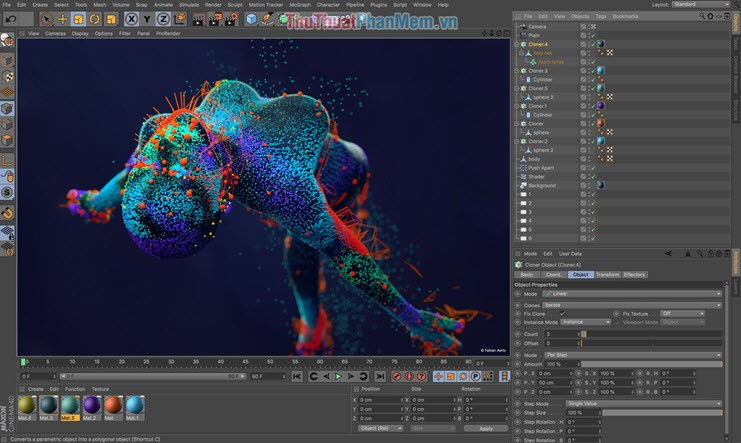
\includegraphics[width=0.7\linewidth]{do_hoa_may_tinh}
			\caption{}
			\label{fig:dohoamaytinh}
		\end{figure}
	\end{frame}
	\begin{frame}
		\begin{figure}
			\centering
			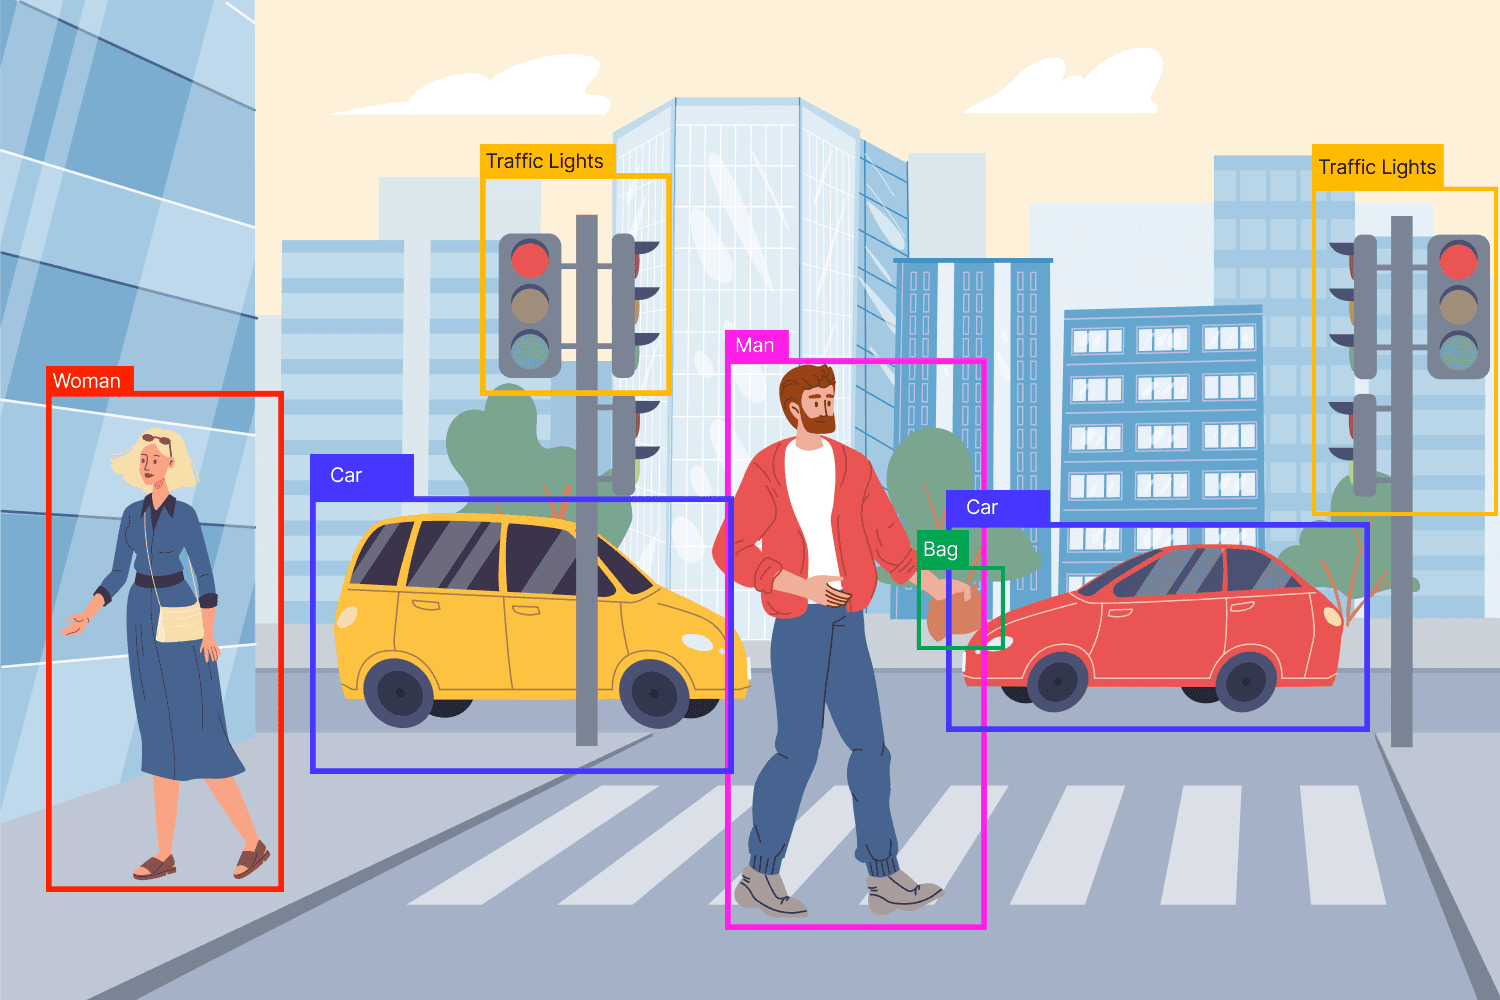
\includegraphics[width=0.7\linewidth]{nhan_dang_mau}
			\caption{}
			\label{fig:nhandangmau}
		\end{figure}
	\end{frame}
	\begin{frame}
		\begin{figure}
			\centering
			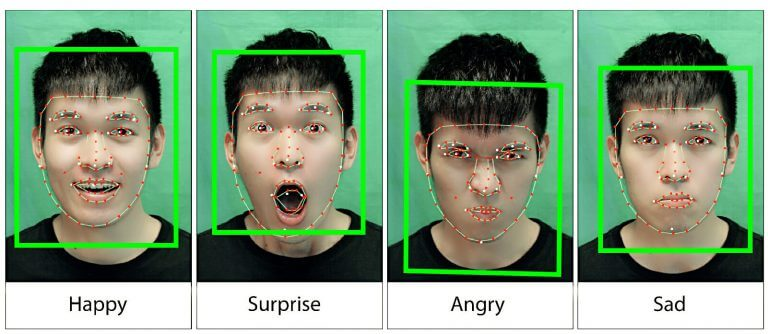
\includegraphics[width=0.7\linewidth]{xu_ly_hinh_anh}
			\caption{}
			\label{fig:xulyhinhanh}
		\end{figure}
		
	\end{frame}
	\begin{frame}
		\begin{figure}
			\centering
			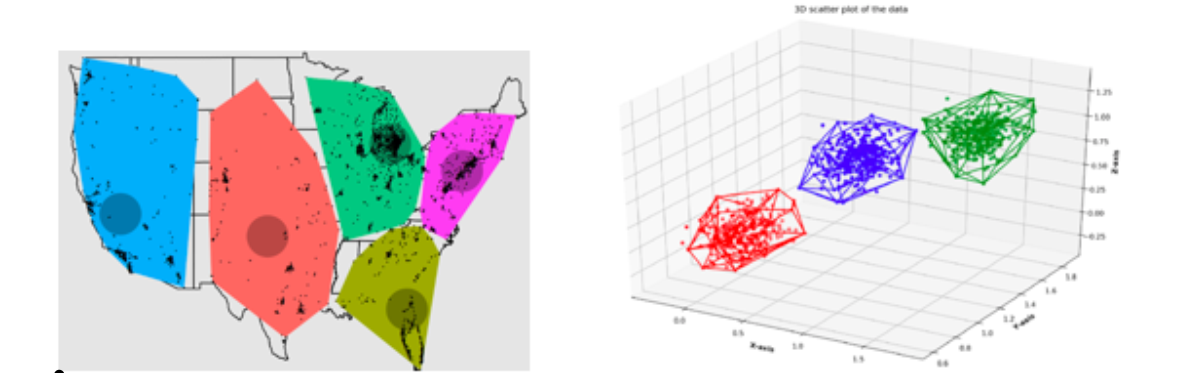
\includegraphics[width=0.7\linewidth]{convex_hull_for_clustering}
			\caption{Covnex hull for clustering}
			\label{fig:convexhullforclustering}
		\end{figure}
		
		\end{frame}
		\begin{frame}
			\begin{figure}
				\centering
				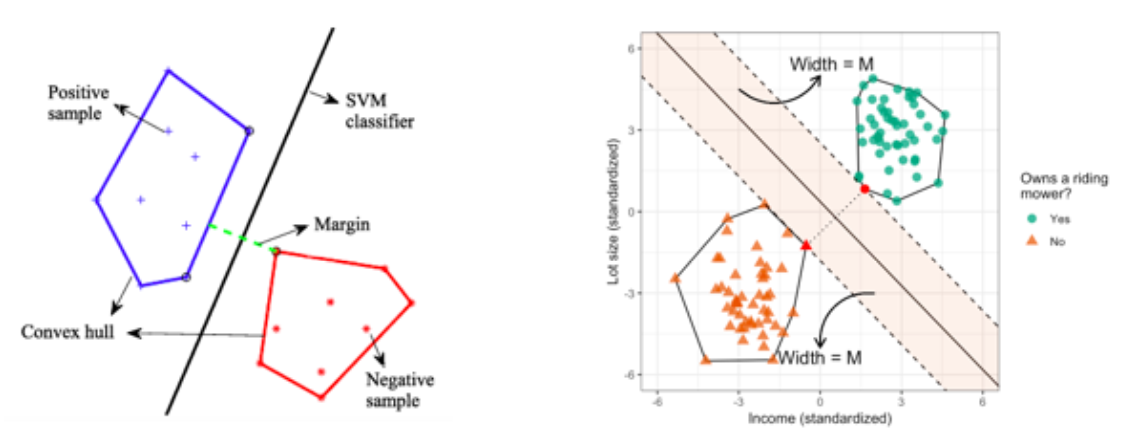
\includegraphics[width=0.7\linewidth]{convex_hull_for_classification}
				\caption{Convex hull for classification}
				\label{fig:convexhullforclassification}
			\end{figure}
			
		\end{frame}
		\begin{frame}
			\begin{figure}
				\centering
				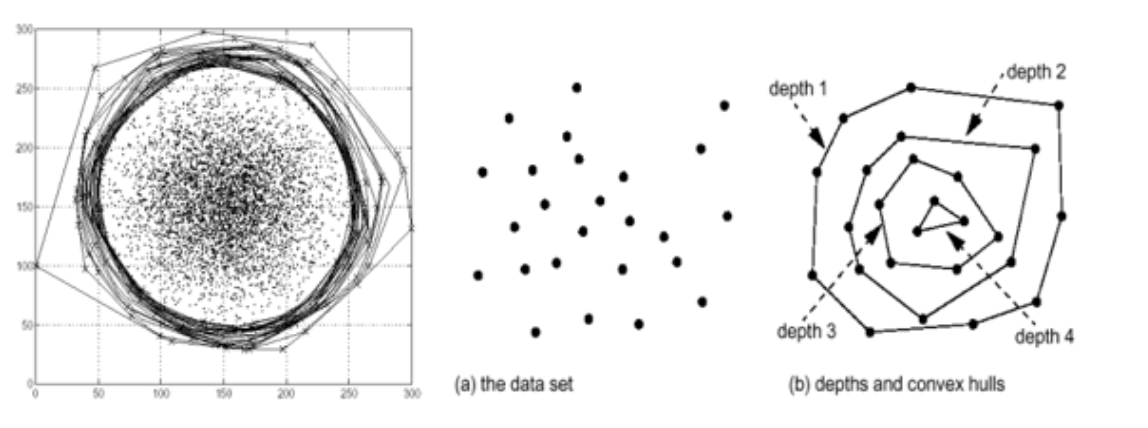
\includegraphics[width=0.7\linewidth]{convex_hull_for_identify_outliers}
				\caption{}
				\label{fig:convexhullforidentifyoutliers}
			\end{figure}
			
		\end{frame}
	\begin{frame}{Tìm bao lồi là một bước tiền xử lý quan trọng trong các bài toán hình học}
	\begin{figure}
		\centering
		
		\begin{subfigure}[b]{0.4\textwidth}
			\centering
			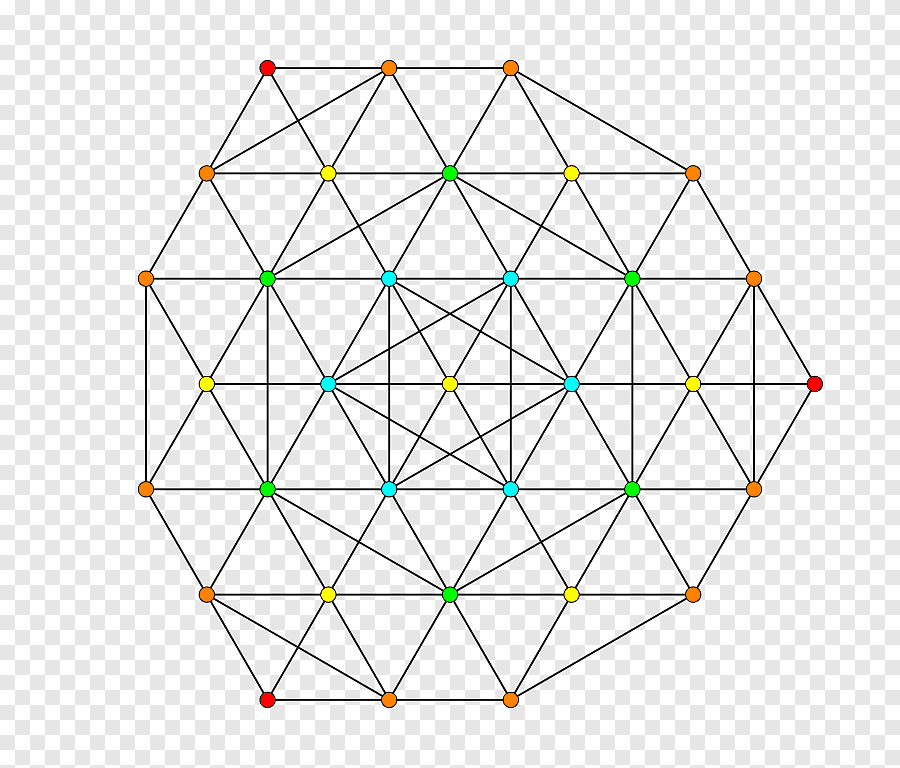
\includegraphics[width=\textwidth]{tam_giac_phan_delauney}
			\caption{Tam giác phân Delaunay}
			\label{fig:tamgiacphandelaunay}
		\end{subfigure}
		\hfill
		\begin{subfigure}[b]{0.4\textwidth}
			\centering
			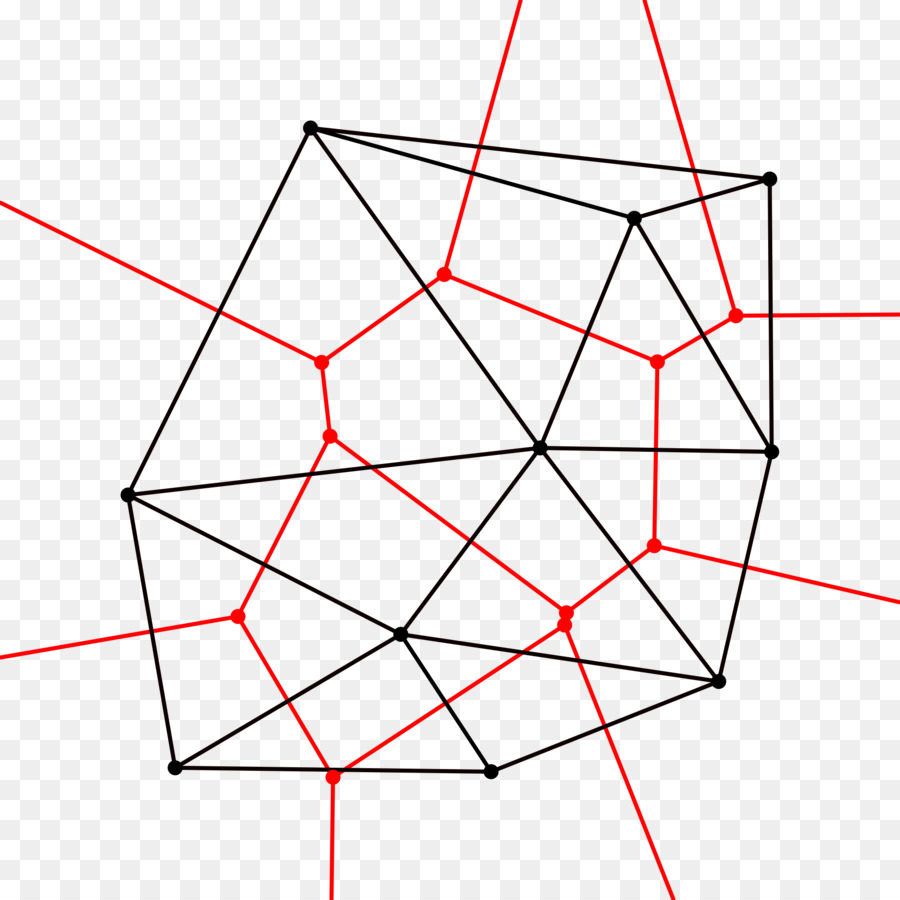
\includegraphics[width=\textwidth]{bieu_do_voronoi}
			\caption{Biểu đồ Voronoi}
			\label{fig:bieudovoronoi}
		\end{subfigure}
		\label{fig:boitrihaihinh}
	\end{figure}
	\end{frame}
	\subsection{Ứng dụng của bao lồi xấp xỉ}
	\begin{frame}
		\begin{itemize}
				\item Giảm thời gian tính toán so với bao lồi chính xác.
				\item Không thể tính toán bao lồi chính xác với dữ liệu không chính xác, không đầy đủ, hoặc chứa nhiễu.
			\end{itemize}
	\end{frame}
	\subsection{Ứng dụng của bao lồi trực giao}
	\section{Thuật toán tính bao lồi xấp xỉ}
	\subsection{Kiến thức ban đầu}
	\begin{frame}{Giới thiệu}
		Thuật toán xấp xỉ sử dụng khoảng cách Hausdorff là một công cụ được dùng để tính toán khoảng cách giữa hai tập hợp bao lồi.
		Thuật toán sử dụng tham số $\delta$ kết hợp để tuỳ chỉnh xấp xỉ bao lồi.(cái này để tự nói hơn).\\
			Định nghĩa bao lồi xấp xỉ:
		\begin{equation}
			\mathcal{P}^{outer} := \{x \in \mathbb{R}^2 \ | \ d x^T \leq \beta_d \text{ với tất cả } d \in D\}
		\end{equation}
	\end{frame}	
		\subsection{Thuật toán xấp xỉ lồi ngoài}



	
	\begin{frame}{Khởi tạo ban đầu}
			\begin{center}
			Định nghĩa đường thẳng $[x; x'] := \{(1 - \lambda)x + \lambda x' | \lambda \in [0; 1]\}$.\\
		\end{center}
		Cho tập hợp điểm không cùng nằm trên 1 đường thẳng.
		
	
		=> Cần tìm một bao lồi xấp xỉ lồi ngoài $\mathcal{P}^{outer}$ sao cho: 
		\begin{center}
			$dist_H(conv X; P^{outer}) \leq \delta$
		\end{center}
			\begin{center}
				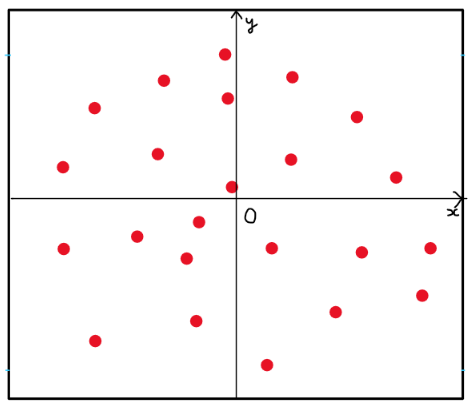
\includegraphics[width=4cm]{Figures/khoi_tao_tap_diem}
			\end{center}
	\end{frame}
	\begin{frame}{Bắt đầu thuật toán}
		Khởi tạo hình chữ nhật lớn nhất bao quanh các điểm.
		\begin{figure}
			\label{fig:khoitaohcnbaoquanh}
			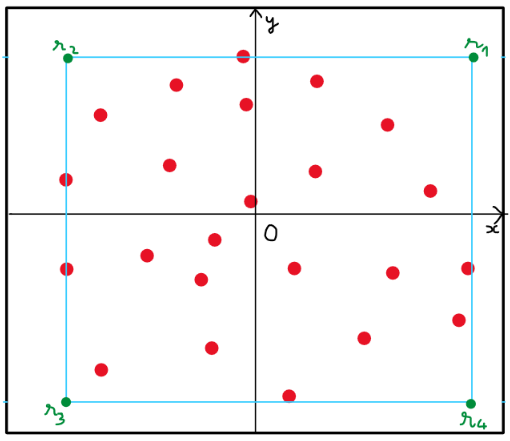
\includegraphics[width=6cm]{Figures/khoi_tao_hcn_bao_quanh}
		\end{figure}
	\end{frame}
	\begin{frame}
		Hình chữ nhật $\mathcal{P}^{outer}$ cấu tạo gồm 4 đỉnh như sau:
		Tập P ban đầu chứa 4 đỉnh này:\\
		\begin{equation}\label{def_4r-2}
			P := \{r_1,\ r_2,\ r_3,\ r_4\}
		\end{equation}
			Lấy 1 đỉnh $p \in P$.\\
		$p^{-}$ là điểm liền trước (ngược chiều kim đồng hồ) của $p$,\\
		$p^{+}$ là điểm liền sau của $p$,\\
	\end{frame}
	\begin{frame}
	
		 ta tính được:\\
		\begin{equation}\label{def_d_p}
			\begin{array}{lcl}
				d_{p}^T &:=& \|p^+ - p^-\|^{-1}\, R \, (p^+ - p^-)^T, \\
				\beta_{d_{p}} &:=& \max\{d_{p}\, x^T \mid x \in X\},
			\end{array}
		\end{equation}
		Với $R$ là ma trận xoay 2 x 2 theo chiều kim đồng hồ.\\
		Xét biểu thức định nghĩa $\mathcal{P}^{outer}$:
		\begin{equation}\label{pt15}
			d_p\, x^T \leq \beta_{d_p}.
		\end{equation}
	\end{frame}
	\begin{frame}{Trường hợp 1}
		
		Nếu:
		\begin{equation}
			\label{betaequal}
			\beta_{d_p} = d_p\, p^+
		\end{equation}
		Thì ràng buộc (\ref{pt15}) sẽ không tạo đỉnh mới mà tạo thêm cạnh mới $[p^-, p^+]$ của $\mathcal{P}^{outer}$.\textit{ (đoạn này phải hỏi cô)}Cho $d_{[p^-, p]}$ và $d_{[p, p^+]}$ là hai hướng cực đại từ $D$ định nghĩa hai cạnh $[p^-, p]$ và $[p, p^+]$ của đa giác $\mathcal{P}^{outer}$. Sau đó hai cạnh này trở nên thừa ra: (đoạn này có thể nói mồm được).
			\begin{equation}\label{newDP2}
			\begin{array}{lcl}
				D &:=& (D \cup \{d_{p}\})\setminus \{d_{[p^-,p]}, d_{[p,p^+]}\}, \\
				P &:=& P \setminus \{p\}.
			\end{array}
		\end{equation}
	\end{frame}
	\begin{frame}{Trường hợp 2}
		 Nếu:
		\begin{equation}\label{betagreater}
			\beta_{d_p} > d_p\, p^+
		\end{equation}
		và:
		\begin{equation}\label{greaterdelta}
			d_{p}\, p^T - \beta_{d_{p}} > \delta
		\end{equation}
		=> ràng buộc (\ref{pt15}) tạo thêm 2 đỉnh mới $\hat p^-$ và $\hat p^+$:
	
			\begin{equation}\label{def_hatp}
				\begin{array}{lcl}
					\lambda_p &:=& (\beta_{d_p} - d_p\, p^{-T})/(d_p\, p^T - d_p\, p^{-T}) \in (0, 1), \\
					\hat p^- &:=& (1 - \lambda_p)\, p^{-T} + \lambda_p\, p^T, \\
					\hat p^+ &:=& (1 - \lambda_p)\, p^{+T} + \lambda_p\, p^T.
				\end{array}
			\end{equation}
		
	\end{frame}
	
	\begin{frame}
		Thêm $d_p$ vào $D$, thay thế $p \in P$ bởi $\hat p^+$ và $\hat p^+$:
		\begin{equation}\label{newDP1}
			\begin{array}{lcl}
				D &:=& D \cup \{d_{p}\}, \\
				P &:=&(P \setminus \{p\}) \cup \{\hat p^-, \hat p^+\}.
			\end{array}
		\end{equation}
		
	\end{frame}
	
\begin{frame}{Một vài kết quả của xấp xỉ lồi ngoài}
	\begin{figure}[htbp]
		\centering
		\begin{subfigure}[b]{0.4\textwidth}
			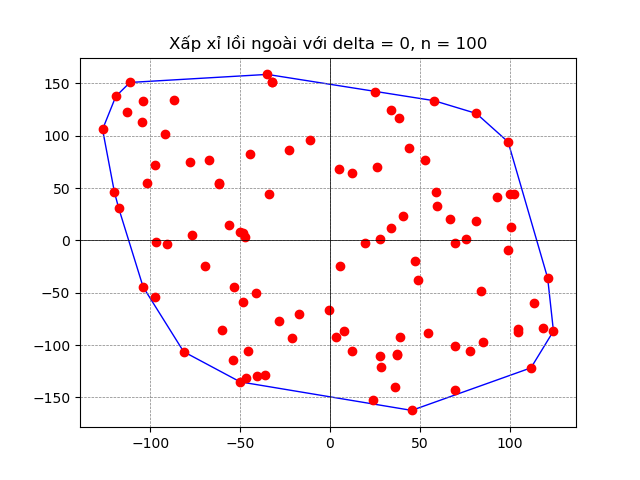
\includegraphics[width=\textwidth]{outer_delta0}
		
			\label{fig:outerdelta0}
		\end{subfigure}
		\hfill
		\begin{subfigure}[b]{0.4\textwidth}
			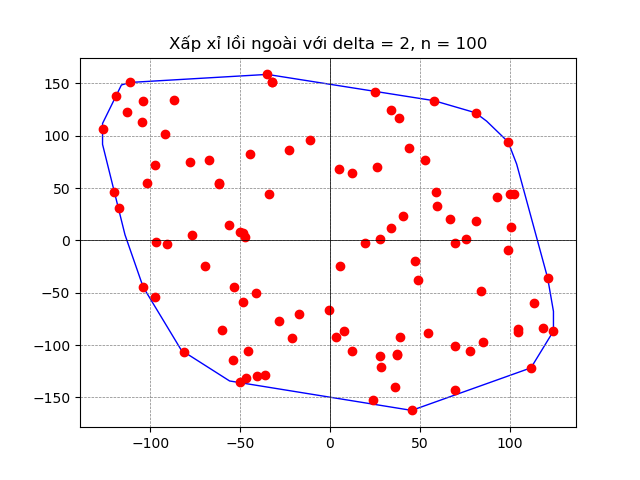
\includegraphics[width=\textwidth]{outer_delta2}
		
			\label{fig:outerdelta2}
		\end{subfigure}
		
		\begin{subfigure}[b]{0.4\textwidth}
			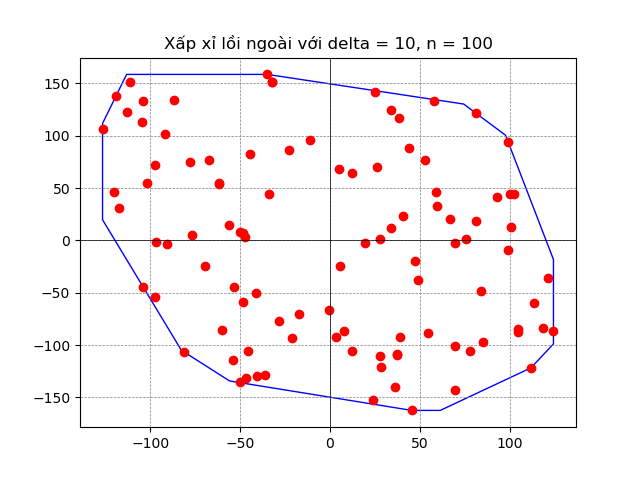
\includegraphics[width=\textwidth]{outer_delta10}
		
			\label{fig:outerdelta10}
		\end{subfigure}
		\hfill
		\begin{subfigure}[b]{0.4\textwidth}
			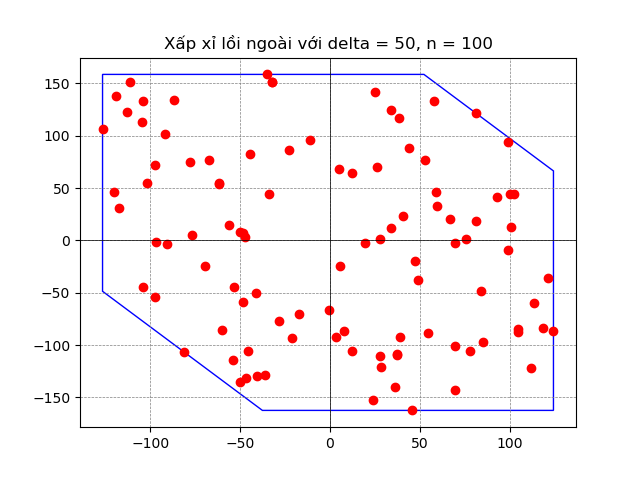
\includegraphics[width=\textwidth]{outer_delta50}
	
			\label{fig:outerdelta50}
		\end{subfigure}
	\end{figure}
\end{frame}

	

	\subsection{Thuật toán bao lồi xấp xỉ trong}
	
	\begin{frame}{Trình bày thuật toán}
		Cho tập $X := {x_1, x_2, ..., x_n} \subset \mathbb{R}^2$
		giả sử $x_1, x_2, ..., x_n$ không cùng nằm trên 1 đường thẳng.\\
		Cần tìm một bao lồi xấp xỉ trong của $\mathcal{P}^{inner}$:
		\begin{equation}\label{ct2.37}
			{\cal P}^{\rm inner} := \ conv \ X', \ \mbox{ với } X' \subset X,
		\end{equation}
	\end{frame}
	\begin{frame}{Xấp xỉ lồi trong}
		Xét hai công thức:\\
		\begin{equation}\label{ct2.40}
			\begin{array}{lcl}
				X' &:=& \{\bar q_1, \bar q_2, \bar q_3, \bar q_4\}, \\
				E &:=& \{[\bar q_1, \bar q_2], \, [\bar q_2, \bar q_3], \, [\bar q_3, \bar q_4], \, [\bar q_4, \bar q_1]\},
			\end{array}
		\end{equation}
		"$\bar q_1 \text{: điểm có giá trị y lớn nhất trong tập các điểm có x lớn nhất}$",
		"$\bar q_2 \text{: điểm có giá trị x nhỏ nhất trong tập các điểm có y lớn nhất}$",
		"$\bar q_3 \text{: điểm có giá trị y nhỏ nhất trong tập các điểm có x nhỏ nhất}$",
		"$\bar q_4 \text{: điểm có giá trị x lớn nhất trong tập các điểm có y nhỏ nhất}$",
	\end{frame}
	\begin{frame}
		\begin{figure}
			\centering
			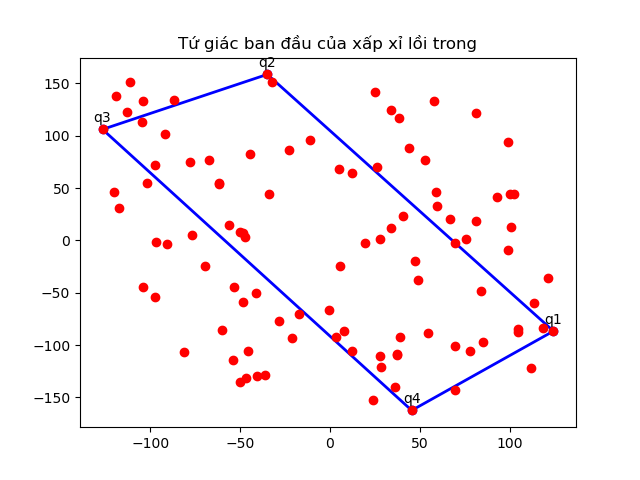
\includegraphics[width=0.7\linewidth]{initial_polygon_inner}
			\caption{Tứ giác khởi tạo ban đầu xấp xỉ lồi trong.}
			\label{fig:initialpolygoninner}
		\end{figure}
	\end{frame}
	\begin{frame}
		Xét cạnh bất kỳ $[p, p^+] \in E$ ($p \not= p^+$), xác định:
		\begin{equation}\label{ct2.44}
			\begin{array}{lcl}
				\bar d_{[p, p^+]}^{\, T} &:=& \|p^+ - p\|^{-1} R \, (p^+ - p)^T, \\
				X_{[p, p^+]} &:=& \{x \in X \mid \bar d_{[p, p^+]}\, x^T > \bar d_{[p, p^+]}\, p^T \},
			\end{array}
		\end{equation}
		Với $R$ là ma trận xoay ngược chiều theo hướng kim đồng hồ.\\
		 Chú ý rằng, ma trận xoay trong thuật toán tìm bao lồi xấp xỉ trong ngược với ma trận xoay ở thuật toán tìm bao lồi xấp xỉ ngoài. 
	\end{frame}
	\begin{frame}
		Nếu $X_{[p, p^+]} \not= \emptyset$ thì xác định:
		\begin{equation}\label{ct2.45}
			\begin{array}{lcl}
				\beta_{[p, p^+]} &:=& \max \{\bar d_{[p, p^+]}\, x^T \mid x \in X_{[p, p^+]}\}, \\
				B_{[p, p^+]} &:=& \{x \in X_{[p, p^+]} \mid \bar d_{[p, p^+]}\, x^T = \beta_{[p, p^+]}\}.
			\end{array}
		\end{equation}
			Nếu:
		\begin{equation}\label{dct2.46}
			\beta_{[p, p^+]} - \bar d_{[p, p^+]}\, p^T \leq \delta
		\end{equation}
		Thì không cần phải mở rộng ${\cal P}^{\rm inner }$ theo hướng $\bar d_{[p, p^+]}$ nữa.
	\end{frame}
	\begin{frame}
	Ngược lại, nếu:
	\begin{equation}\label{ct2.47}
		\beta_{[p, p^+]} - \bar d_{[p, p^+]}\, p^T > \delta
	\end{equation}
	thì xác định điểm:
	\begin{equation}\label{ct2.48}
		\hat p \in B_{[p, p^+]} \hbox{ thỏa mãn } \|\hat p - p\| = \max\{\|x - p\| \mid x \in B_{[p, p^+]}\},
	\end{equation}
		Và cập nhật $X'$ và $B$ bởi
	\begin{equation}\label{ct2.49}
		\begin{array}{lcl}
			X' &:=& X' \cup \{\hat p\}, \\
			E &:=& E \cup \{[p, \hat p], \, [\hat p, p^+]\},
		\end{array}
	\end{equation}
	\end{frame}

	\begin{frame}
	Và xác định: 
	\begin{equation}\label{ct2.50}
		\begin{array}{lcl}
			X_{[p, \hat p]} &:=& \{x \in X_{[p, p^+]} \mid \bar d_{[p, \hat p]}\, x^T > \bar d_{[p, \hat p]}\, p^T \}, \\
			X_{[\hat p, p^+]} &:=& \{x \in X_{[p, p^+]} \mid \bar d_{[\hat p, p^+]}\, x^T > \bar d_{[\hat p, p^T]}\, {\hat p}^T \}.
		\end{array}
	\end{equation}
	\end{frame}
\begin{frame}
	\begin{figure}[htbp]
		\begin{subfigure}[b]{0.4\textwidth}
			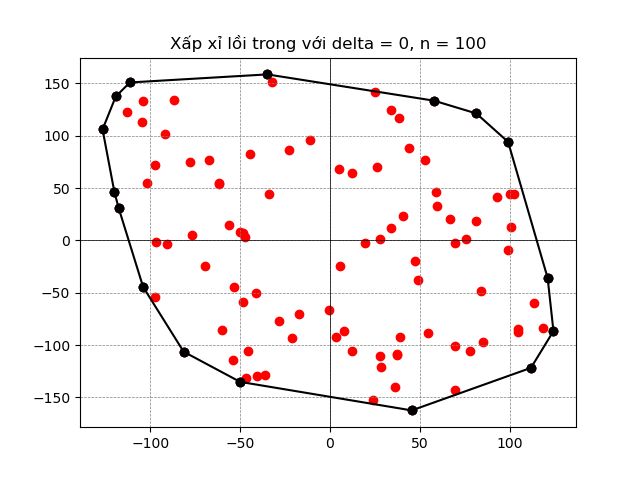
\includegraphics[width=\textwidth]{inner_delta0}
			\label{fig:inner_delta0}
		\end{subfigure}
		\hfill
		\begin{subfigure}[b]{0.4\textwidth}
			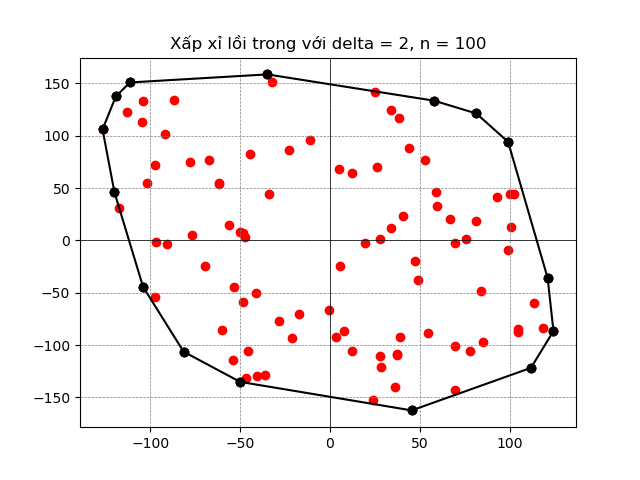
\includegraphics[width=\textwidth]{inner_delta2}
			\label{fig:inner_delta2}
		\end{subfigure}
		
		\begin{subfigure}[b]{0.4\textwidth}
			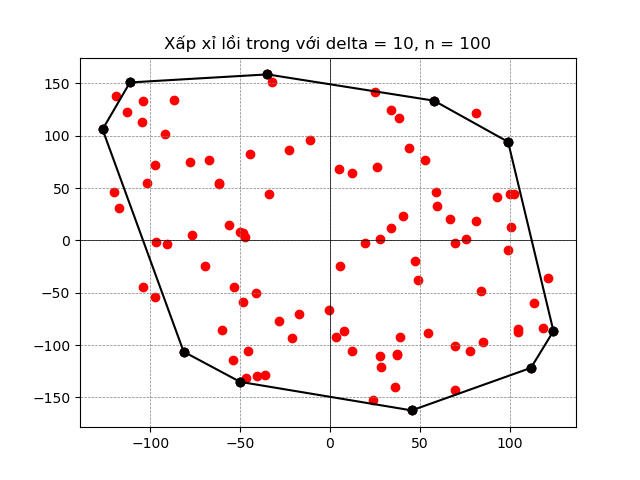
\includegraphics[width=\textwidth]{inner_delta10}
			\label{fig:inner_delta10}
		\end{subfigure}
		\hfill
		\begin{subfigure}[b]{0.4\textwidth}
			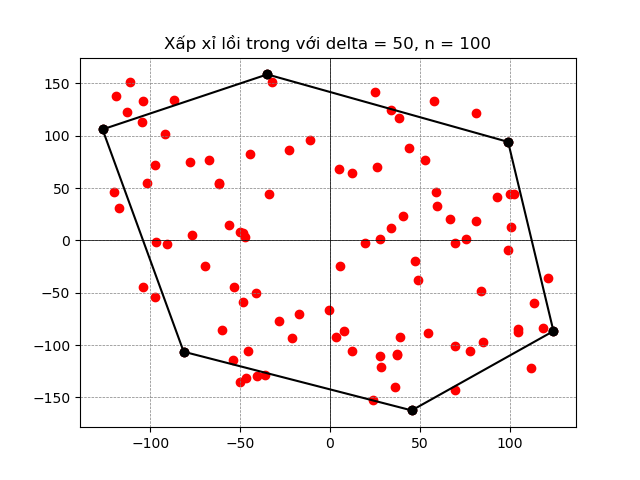
\includegraphics[width=\textwidth]{inner_delta50}
			\label{fig:inner_delta50}
		\end{subfigure}
	\end{figure}
\end{frame}

	\section{Ý tưởng thay thế thuật toán bao lồi xấp xỉ vào một bộ phát hiện}
	\subsection{Giới thiệu chung}
	\begin{frame}{Giới thiệu chung}
			Thách thức lớn: đặc trưng răng cưa (feature aliasing)
			\begin{columns}[c] % Căn giữa các cột
			\column{.5\textwidth} % Cột 1 chiếm 50% của khung
			\begin{figure}
				\centering
				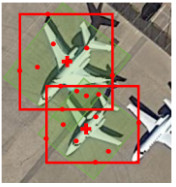
\includegraphics[width=3cm]{reppoint_bouding_box.jpg}
		
			\end{figure}
			\column{.5\textwidth} % Cột 2 chiếm 50% của khung
			\begin{figure}
				\centering
				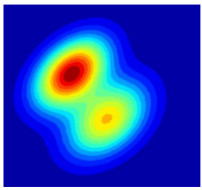
\includegraphics[width=3cm]{reception_field_w_aliasing.jpg}
			
			\end{figure}
		\end{columns}
	\end{frame}
		\begin{frame}{Giới thiệu chung}
		Sử dụng bao lồi làm biểu diễn bounding box.
		\begin{columns}[c] % Căn giữa các cột
			\column{.5\textwidth} % Cột 1 chiếm 50% của khung
			\begin{figure}
				\centering
				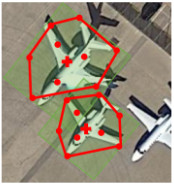
\includegraphics[width=3cm]{ConvexHull_Bouding_Box.jpg}
			
			\end{figure}
			
			\column{.5\textwidth} % Cột 2 chiếm 50% của khung
			\begin{figure}
				\centering
				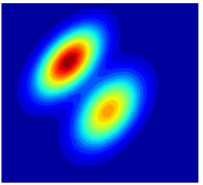
\includegraphics[width=3cm]{reception_field_wo_aliasing.jpg}
			
			\end{figure}
		\end{columns}
	\end{frame}
	\subsection{Ý tưởng thay thế bao lồi vào bộ phát hiện CFA}
	\begin{frame}{Phương pháp thích ứng bao lồi xấp xỉ (Approximation convex-hull feature adaptation-ACFA)}
	 
	 Giới hạn phạm vi đối tượng sử dụng chỉ số ACIoU.\\
	 Phân chia tập bao lồi thành bao lồi xấp xỉ âm và dương.
		\begin{figure}[htp]
			\begin{center}
				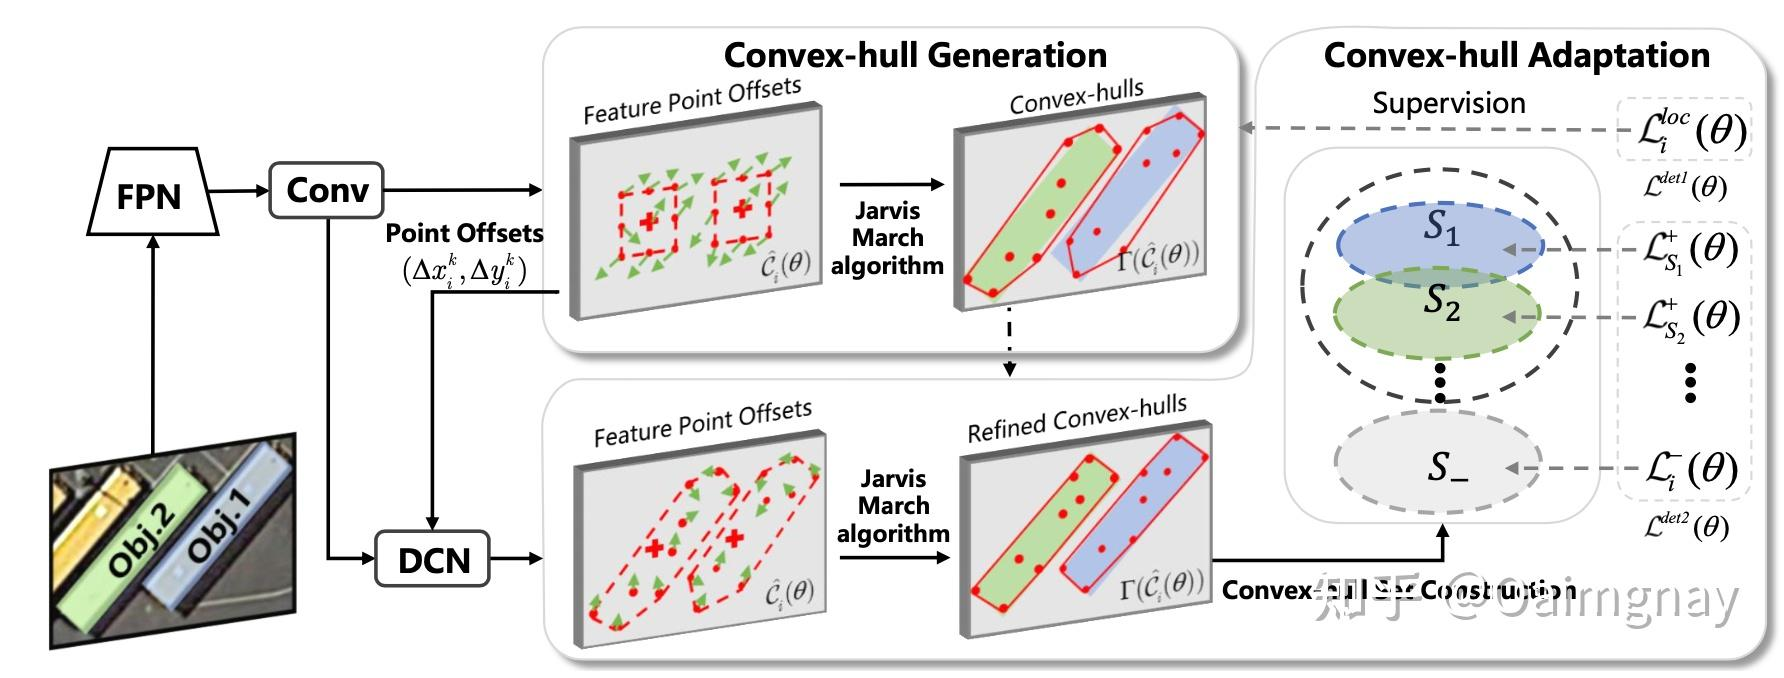
\includegraphics[width=10cm]{./Hinh_1.jpg}
			\end{center}
		\end{figure}
	\end{frame}
	\begin{frame}{Xây dựng tập bao lồi}
		Phương pháp ACFA đã đề xuất biểu diễn phạm
		vi của đối tượng bằng bao lồi:\\
		\begin{align} \label{ptdd}
			C_i = \{(x_i^k, y_i^k )\}_i^{k=1,2,...,K}
		\end{align}
		Phương pháp gồm 2 giai đoạn thực hiện:
			\begin{itemize}
			\item[I.] Tạo và ước lượng bố cục bao lồi.
			\item[II.] Chỉnh sửa bao lồi để phù hợp với các đối tượng dày đặc.
		\end{itemize}	
	\end{frame}
\begin{frame}{Giai đoạn I}
	Dự đoán độ lệch:
	\begin{align} \label{ptdd}
		\widehat C_l (\theta) \gets \{(x_i^k + \Delta x_i^k, y_i^k + \Delta y_i^k )\}_i^{k=1,2,...,K}
	\end{align}
	\begin{center}
		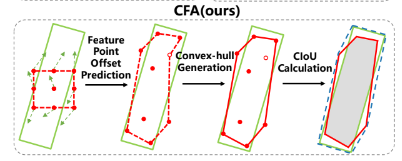
\includegraphics[width=8cm]{Figures/feature_point_offset_prediction}
	\end{center}
\end{frame}
\begin{frame}{Định nghĩa công thức Approximation Convex Intersection over Union (ACIoU)}
		\begin{align} 
			ACIoU_{(C_i (\theta), B_j)} (\theta) = \frac{|C_i(\theta) \cap B_j|}{|C_i(\theta) \cup B_j|} - \frac{|R_j \setminus (C_i(\theta) \cup B_j)|}{|R_j|}
		\end{align}	
		Hàm loss định vị (localization loss):
		\begin{align} \label{ptdd0}
			\mathcal{L}_i^{loc} (\theta) = 1 - ACIoU(C_i(\theta), B_j)
		\end{align}
\end{frame}
	\begin{frame}
		Hàm loss phân loại (classification loss) cho bao lồi dương:\\
		\begin{align} \label{ptdd2}
			\mathcal{L}^+ (\theta) = \mathcal{L}_i^{cls}(S_i(\theta), Y_j) +\lambda 	\mathcal{L}_i^{loc}(C_i(\theta), B_j)
		\end{align}
		Hàm loss phân loại cho bao lồi âm:\\
		\begin{align} \label{ptdd3}
			\mathcal{L}^- (\theta) = \mathcal{L}_i^{cls}(S_i(\theta), Y_j) 
		\end{align}
		
	\end{frame}
	\begin{frame}{Thích ứng bao lồi - Approximation Convex Hull Adaptation}
		Xử lý hiện tượng feature aliasing. \\
		\textbf{Convex-Hull Set Construction}: Xây dựng một tập các bao lồi xấp xỉ cho mỗi đối tượng.
		\begin{figure}[ht!]
			\begin{center}
				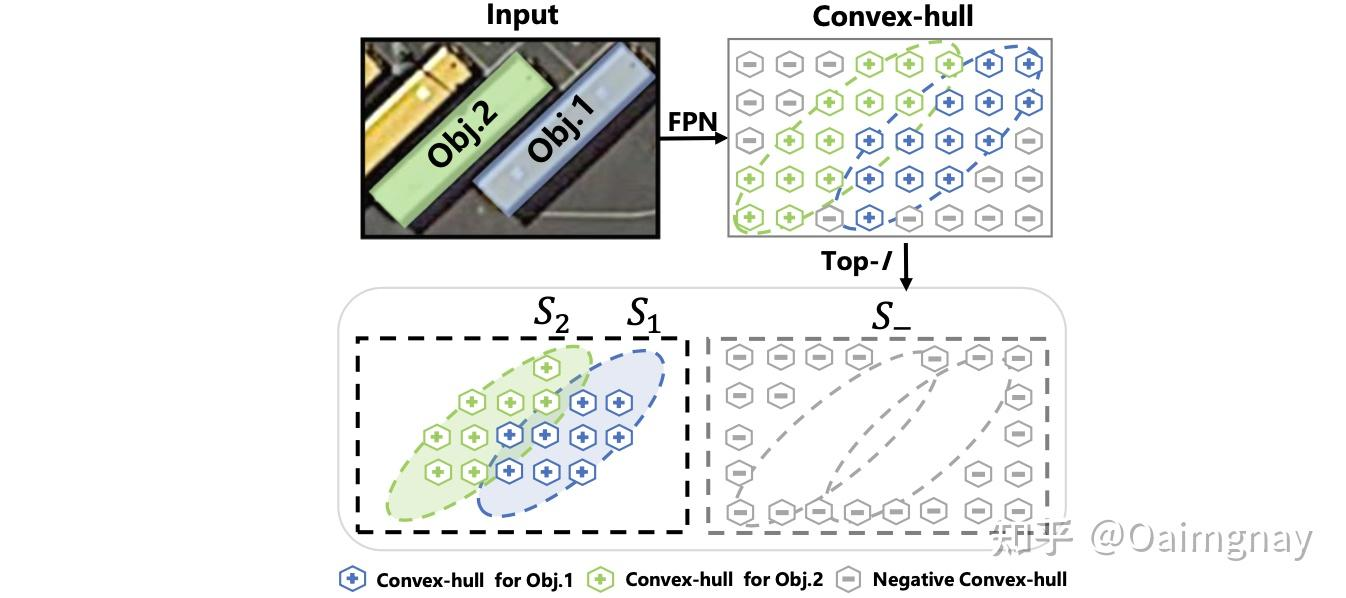
\includegraphics[width=10cm]{./Hinh_8.jpg}
			\end{center}
		\end{figure}
	\end{frame}
	
	\begin{frame}{Xây dựng tập các bao lồi xấp xỉ}
		Tập các bao lồi xấp xỉ dương($S_j$) được xây dựng bằng cách chọn ra \textit{top-I} bao lồi xấp xỉ làm bao lồi xấp xỉ dương, theo ACIoU giữa các bao lồi dự đoán và bao lồi chính xác của đối tượng (grouth-truth).\\
			Cách chia tập các bao lồi được hướng dẫn bởi nguyên tắc nhất quán đạo hàm.
		\begin{align} \label{ptdd7}
			\frac{\partial\mathcal{L}_{S_j}^+ (\theta)}{\partial (\theta)} = \frac{1}{|S_j|} \sum_{i \in {S_j}} \frac{\partial (f(\mathcal{L}_i^+(\theta))\mathcal{L}_i^{+}(\theta))}{\partial (\mathcal{L}_i^+(\theta))} \frac{\partial \mathcal{L}_i^+ (\theta)}{\partial (\theta)}
		\end{align}
	\end{frame}
	\begin{frame}{Chiến lược phân đoạn tập các bao lồi}
		\begin{figure}[ht!]
			\begin{center}
				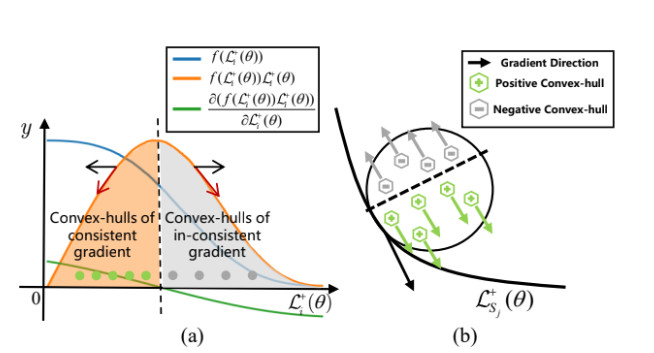
\includegraphics[width=10cm]{./Hinh_9.jpg}
				\caption{Chia tách tập convex-hull dựa trên nguyên tắc tính thống nhất gradient.}
				\label{upper_convex_function}
			\end{center}
		\end{figure}
	\end{frame}
	\begin{frame}{Xử lý hiện tượng đặc trưng răng cưa}
		Đưa ra công thức tính hệ số khử đặc trưng răng cưa:
		\begin{align} \label{ptdd8}
			p_i = \gamma \frac{CIoU (\mathcal{C}_i, \mathcal{B}_j)}{\sum_{m=1}^{M} CIoU (\mathcal{C}_i, \mathcal{B}_m)}
		\end{align}
	
		Nhân hệ số khử này vào hàm loss, ta có hàm loss giai đoạn 2:\\
		\begin{equation}
			\mathcal{L}_{s_j}^{+}(\theta)=\frac{1}{\left|S_j\right|} \sum_{i \in S_j} p_i f\left(\mathcal{L}_i^{+}(\theta)\right) \mathcal{L}_i^{+}(\theta)
		\end{equation}
		
	\end{frame}
	\begin{frame}{Hàm loss của bộ phát hiện CFA}
		Là tổng hàm loss của cả hai giai đoạn:
		\begin{align}
			\mathcal{L}_{CFA} = \mathcal{L}^{\operatorname{det} 1}(\theta)+\mathcal{L}^{\operatorname{det} 2}(\theta)
		\end{align}
		
	\end{frame}
	\section{Một số kết quả thu được}
	\begin{frame}
		
\begin{figure}
	\centering
	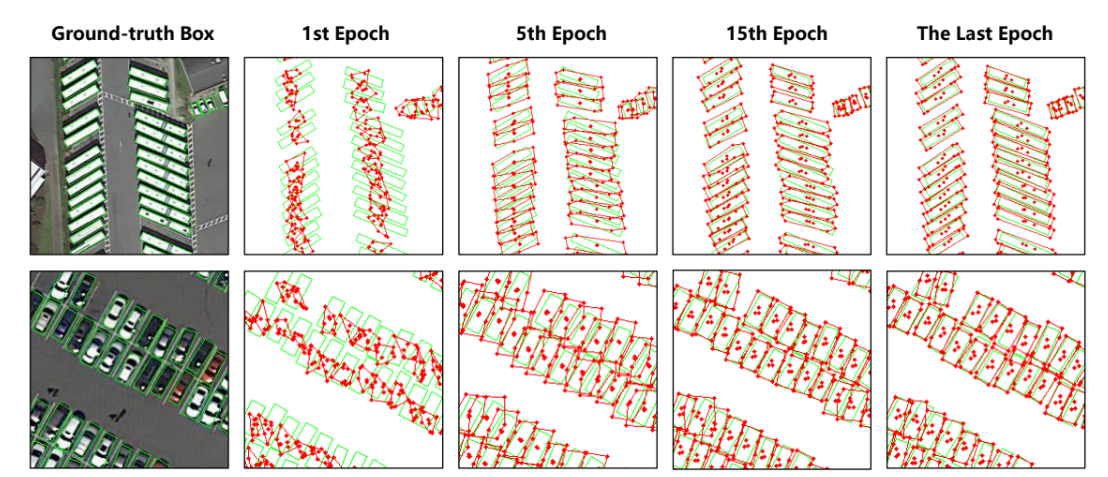
\includegraphics[width=1\linewidth]{Figures/convex_hull_evaluation_when_training}
	\caption{Sự thay đổi của bao lồi trong quá trình huấn luyện.}
	\label{fig:convexhullevaluationwhentraining}
\end{figure}
\end{frame}
	\begin{frame}
\begin{figure}
	\centering
	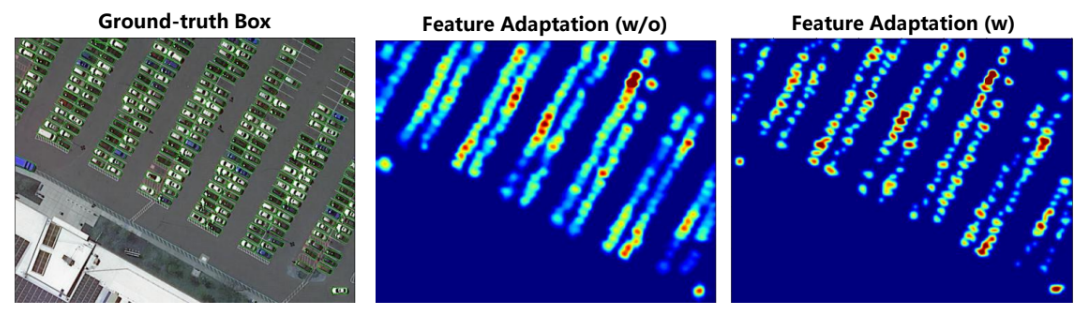
\includegraphics[width=1\linewidth]{Figures/heat_map_comparision_of_CFA}
	\caption{Biểu đồ nhiệt khi có thích ứng bao lồi (phải) và không có thích ứng bao lồi (trái).}
	\label{fig:heatmapcomparisionofcfa}
\end{figure}
		
	\end{frame}
\begin{frame}{Một số kết quả thu được của CFA}
			
	\begin{figure}
		\centering
		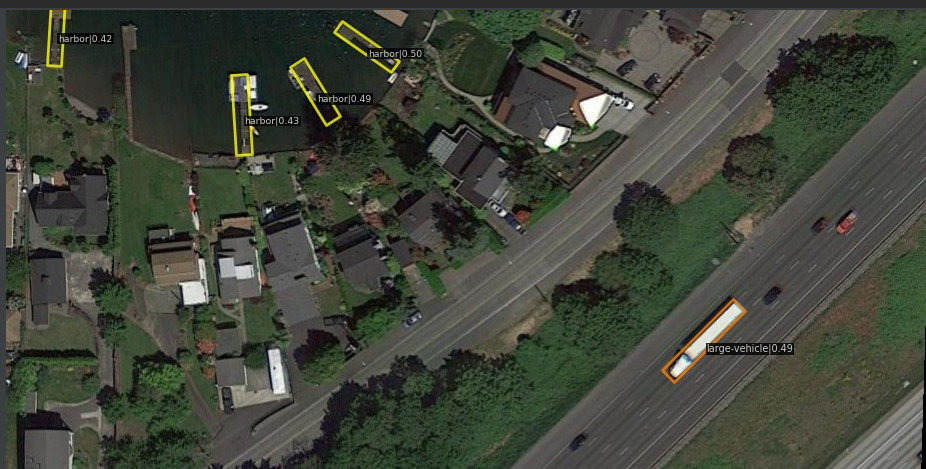
\includegraphics[width=1\linewidth]{res_mmrotate3}
	
		\label{fig:resmmrotate3}
	\end{figure}
\end{frame}
\begin{frame}
	\begin{figure}
		\centering
		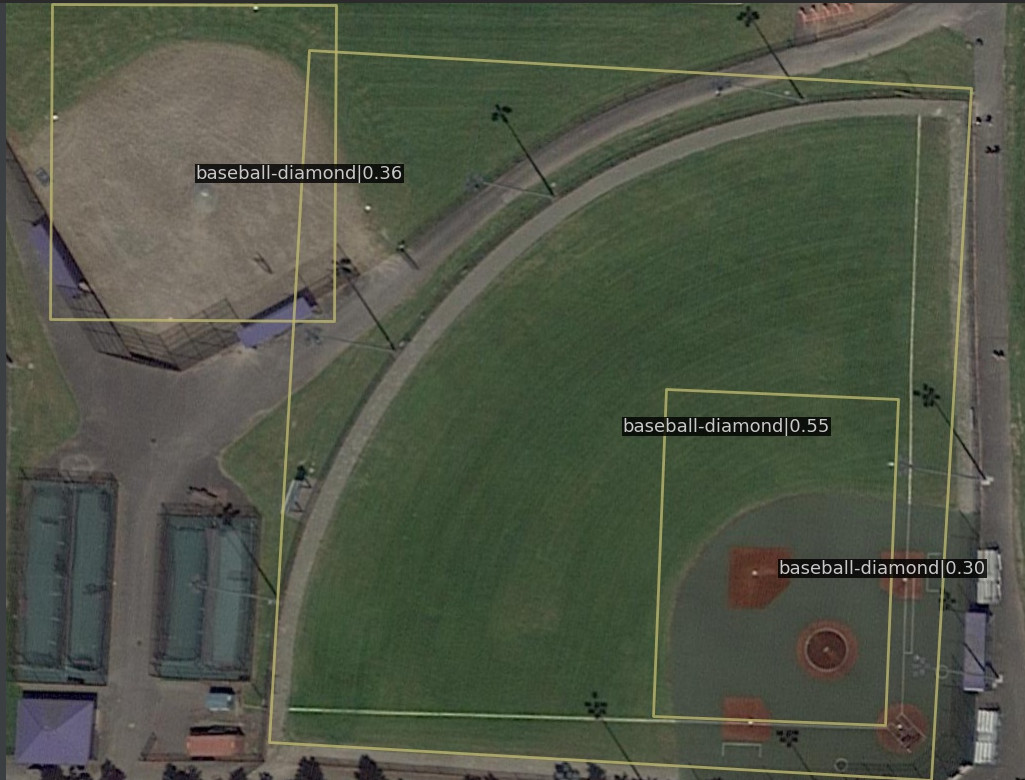
\includegraphics[width=0.8\linewidth]{res_mmrotate4}
	
		\label{fig:resmmrotate4}
	\end{figure}
\end{frame}
\begin{frame}
	\begin{figure}
		\centering
		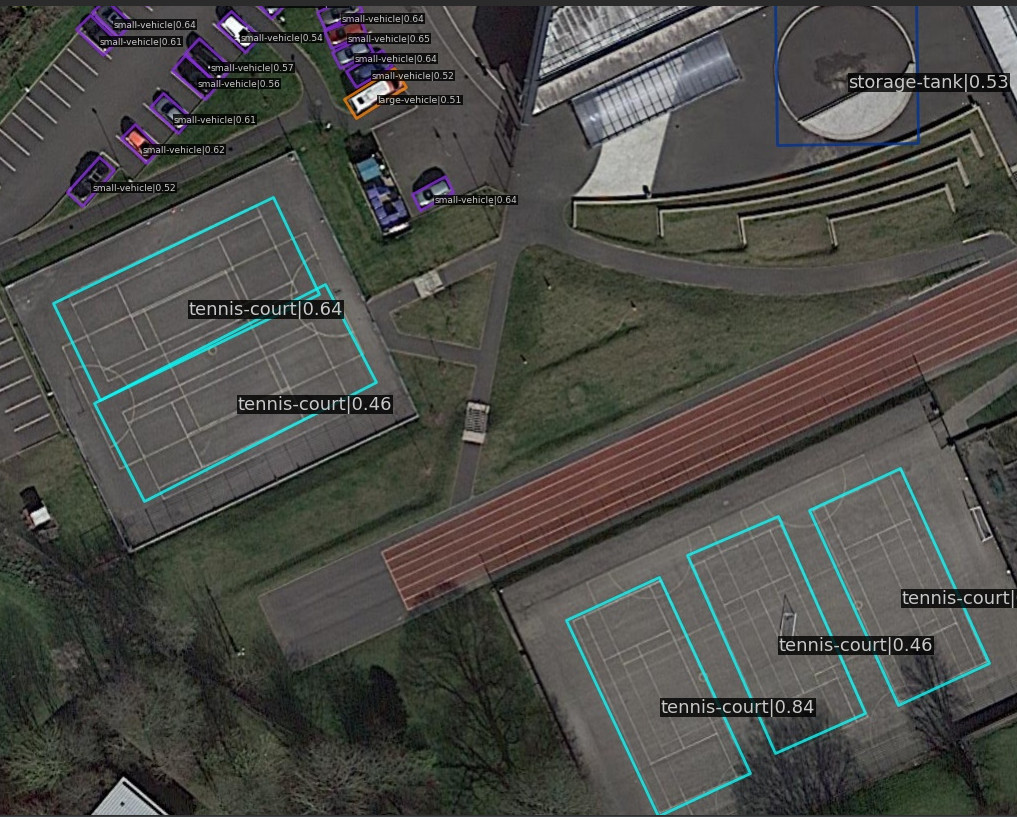
\includegraphics[width=0.9\linewidth]{res_mmrotate5}
	
		\label{fig:resmmrotate5}
	\end{figure}
\end{frame}
\begin{frame}
	\begin{figure}
		\centering
		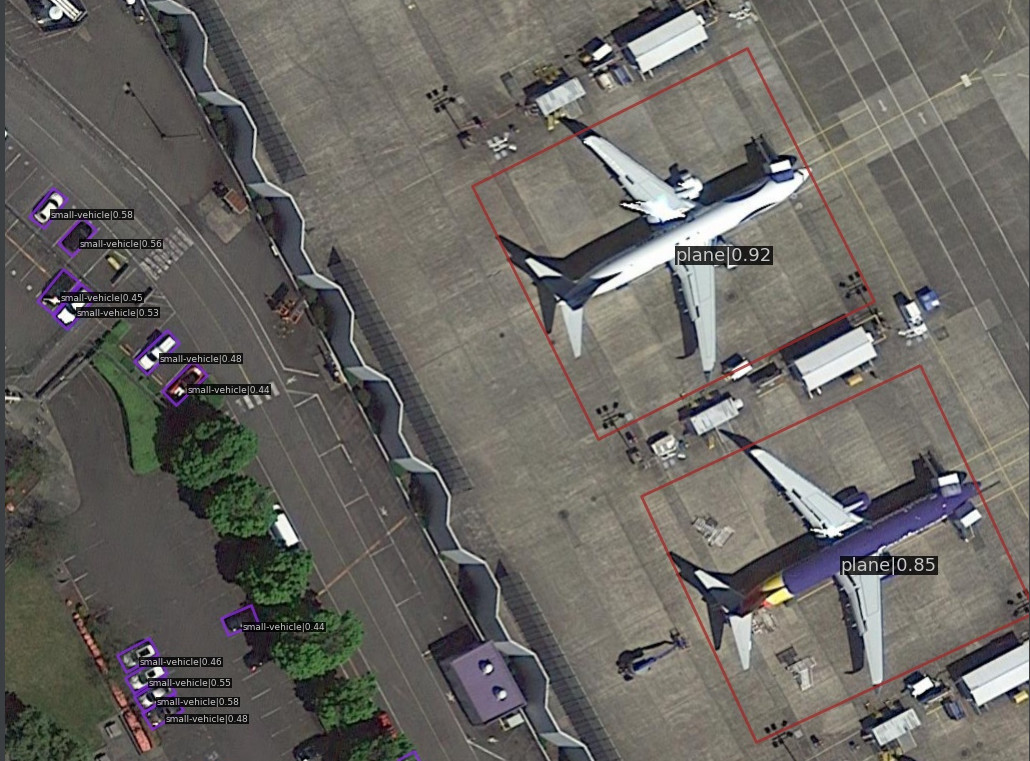
\includegraphics[width=0.9\linewidth]{res_mmrotate2}
		\label{fig:resmmrotate2}
	\end{figure}
\end{frame}

\end{document}
